\documentclass[11pt,letterpaper]{article}
\usepackage{fullpage}
\usepackage[top=1.75cm, bottom=4cm, left=1.25cm, right=1.25cm]{geometry}
\usepackage{amsmath,amsthm,amsfonts,amssymb,amscd}
\usepackage{lastpage}
\usepackage{enumerate}
\usepackage{fancyhdr}
\usepackage{mathrsfs}
\usepackage{xcolor}
\usepackage{graphicx}
\usepackage{listings}
\usepackage{hyperref}
\usepackage{tcolorbox}
\usepackage{bbm}
\usepackage{cite}
\usepackage[numbers]{natbib}

\hypersetup{%
colorlinks=true,
urlcolor=blue,
citecolor=blue
}

\renewcommand\lstlistingname{Algorithm}
\renewcommand\lstlistlistingname{Algorithms}
\def\lstlistingautorefname{Alg.}

\lstdefinestyle{Python}{
  language        = Python,
  frame           = lines,
  basicstyle      = \footnotesize,
  keywordstyle    = \color{blue},
  stringstyle     = \color{green},
  commentstyle    = \color{red}\ttfamily
}

\setlength{\parindent}{0.0in}
\setlength{\parskip}{0.05in}

\newtcolorbox{cbox}[3][]
{
  colframe = #2!25,
  colback  = #2!10,
  coltitle = #2!20!black,
  title    = {#3},
  #1,
}

\newcommand\course{CS 674}
\newcommand\instructor{Dr. Wingate}
\newcommand\name{Jake Callahan, Taylor Paskett}

\pagestyle{fancyplain}
\headheight 32pt
\lhead{\name \\ \today}
\chead{\textbf{}}
\rhead{\course \\ \instructor}
\lfoot{}
\cfoot{}
\rfoot{\small\thepage}
\headsep 1.5em

\title{Analyzing Information Loss of Invertible Variational Autoencoders}
\author{\name}

\begin{document}

\maketitle

\section{Introduction}
As we gain access to more and more unstructured data, unsupervised learning methods become more and more vital.
Among existing unsupervised deep learning models, variational autoencoders have become prominent.
An autoencoder uses an unlabelled dataset to create more compactly encoded representations of the dataset.
This is done by introducing a bottleneck to the architecture, as the following image (courtesy of \cite{bottleneck_picture}) depicts:
\begin{figure}[!htb]
\begin{center}
   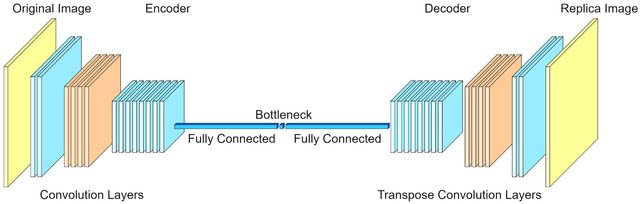
\includegraphics[width=0.65\linewidth]{./pics/bottleneck.jpg}
   \caption{Illustration of Bottleneck in Autoencoder}
\end{center}
\end{figure}

Traditionally, autoencoders are trained by requiring that the original image and the replica image are nearly the same, measured using a reconstruction loss \cite{VAEtutorial}.
After training, we can extract an encoded version of a test image by inputting the test image to the encoder and extracting the value at the bottleneck layer.

More recently, information-theoretic concepts such as mutual information and entropy have been used to better understand autoencoders \cite{infotheoretic_vaes}; and in some cases, information-theoretic concepts can even be used in place of gradient descent to train neural networks \cite{deep_infomax}.

Since information theory helps us understand and train autoencoders, we are interested in studying the information-theoretic properties of a new type of autoencoder that is built using invertible neural networks (INNs).

\section{Invertible Autoencoders}
We examine the work of Nguyen, Ardizzone, and K\"{o}the, in their paper, "Training Invertible Neural Networks as Autoencoders" \cite{Nguyen2019}.

In the following figure from Nguyen et al's work, they explain the fundamental building block of INNs: the invertible coupling layer.
Just like a ResNet is built by stacking residual blocks, INNs are built by stacking invertible coupling layers.
Theoretically, an INN can be built to any depth by stacking any number of invertible coupling layers.

\begin{figure}[!htb]
\begin{center}
   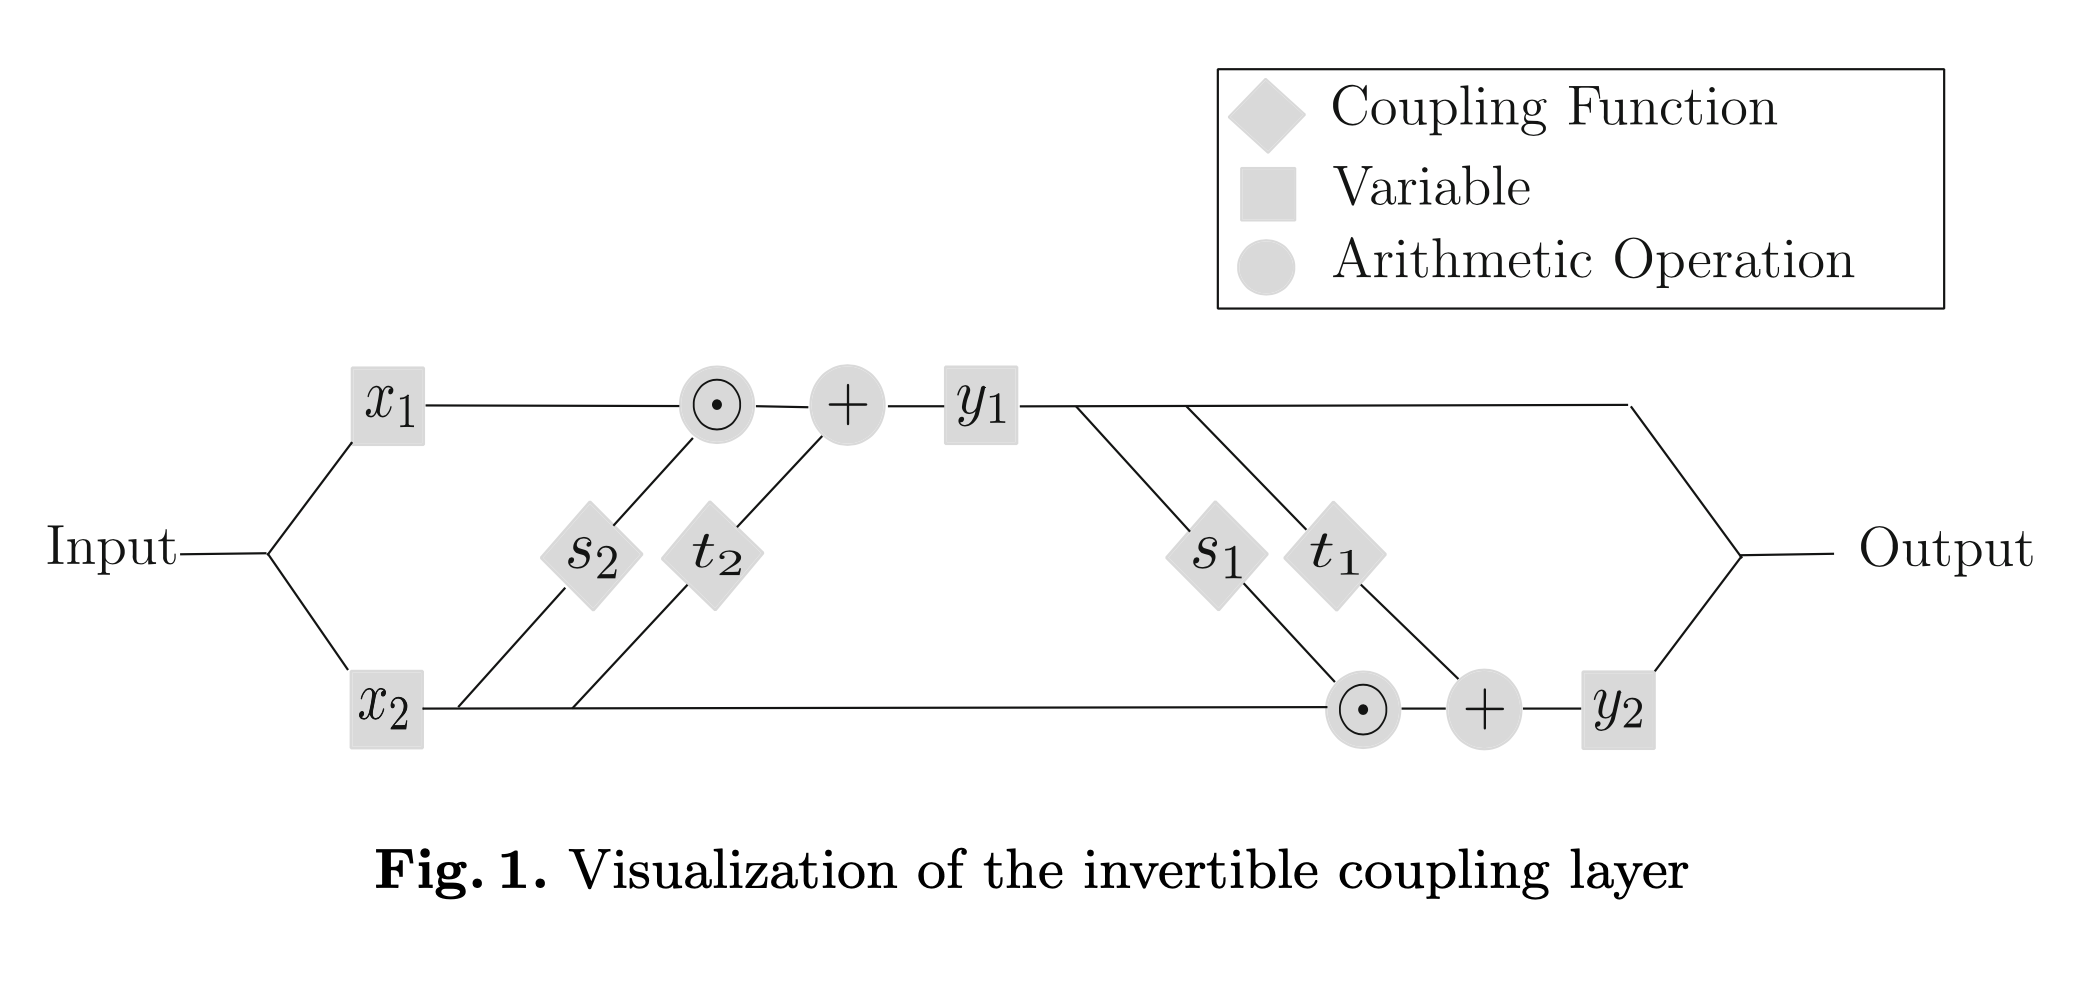
\includegraphics[width=0.8\linewidth]{./pics/invertible_coupling_layer.png}
   \caption{Visualization of the Invertible Coupling Layer}
\end{center}
\end{figure}

Although traditional neural networks are universal function approximators, INNs are limited to approximating bijective functions.
The question you might be asking, then, is this: if INNs can only approximate bijective functions, how can an INN become an autoencoder?
Since the point of an autoencoder is to encode data in a smaller-dimensional latent space, a bijection won't work, right?

The main contribution of Nguyen, et al. was to come up with a creative solution to this problem.
They do so by "zero-padding" the output of the INN.
For example, suppose our inputs have a dimension of 1000, and we wish to create a bottleneck of size 20.
To train our INN, we give it the input $ x $, obtaining $ \text{INN}(x) = y $.
Then, we replace all but the first 20 entries of $ y $ with zero, call this new output $ \hat{y} $.
Finally, we run the inverse model: $\text{INN}^{-1}(\hat{y}) = \hat{x}$.
Then, we seek to minimize the reconstruction loss \begin{align*}
    \mathscr{L}(x, \hat{x}).
\end{align*}
In so doing, we have effectively created a bottleneck.
The zero-padded $ \hat{y} $ has only 20 nonzero entries, and these entries can be thought of as our latent space encoding.

Nguyen et al. obtained very promising results.
Testing with MNIST, CIFAR-10, and CelebA, they showed that, compared to traditional autoencoders: \begin{enumerate}
   \item INNs required less training epochs;
   \item INNs could achieve better reconstruction losses across most bottleneck sizes;
   \item INNs required less trainable parameters than their classic autoencoder counterparts.
\end{enumerate}
The reason for 3 is primarily because the INN architecture is constant with respect to the bottleneck size, where classic autoencoders must change the number of trainable parameters depending on the bottleneck size. In their discussion of their results, they hypothesize the following:
\begin{quotation}
   We already established, that if a DNN does not learn a bijective function, information loss occurs during the forward process making the inverse process ambiguous. The INN solves this ambiguity problem by introducing latent variables z containing all the information lost during the forward process.... Therefore, we hypothesize that INNs have no intrinsic information loss contrary to DNNs and the findings of Yu et al. do not apply to INNs. In other words, INNs are not bound to a maximal number of layers (depth) after which only suboptimal results can be achieved.
\end{quotation}
This is a bold hypothesis, and we will investigate it using information theory.
Primarily, we seek to answer the following questions: \begin{itemize}
   \item How much information entropy is gained or lost at each layer of an INN?
   \item What about a classic autoencoder?
   \item What is the KL-divergence between the distribution of test inputs and reconstructed outputs?
\end{itemize}


\section{Methods, Results}
\subsection{Methods}
   \subsubsection{Experimental Setup}
     In order to answer these questions, we utilized the same models and architecture employed by Nguyen et al.
     We chose to compare the information loss across each layer in a classical model with its INN counterpart using two different datasets: MNIST and CIFAR-10. We chose these datasets so that our results could be comparable to the findings of Nguyen et al. Although we hoped to also used the CelebA data to more closely match the process in \cite{Nguyen2019}, computational and time constraints prevented us from examining this dataset as well.

     We were primarily interested in three metrics for each model and dataset: Shannon entropy of the output at each layer, the relative entropy (measured by KL-Divergence) of the input and output at each layer, and the relative entropy of the model input and reconstructed model output. We measured these metrics on four models total: An Invertible Neural Net and a classical autoencoder on the CIFAR-10 dataset, and an Invertible Neural Net and a classical autoendcoder on the MNIST dataset.

     We partitioned the datasets into a training and test set, trained the models, and then exmained our information metrics on the test set to see how much information the models would retain on unseen data. By examining these three metrics, we hoped to find a clear indicator of whether or not INNs limit information loss to a higher degree than classical autoencoders.

   \subsubsection{Model Architecture}
     In general, we used the extremely well-designed model code and architecture provided by Nguyen et al. and FrEIA. The only modification we made was adding the ability to track layer output at each layer in FrEIA's ReversibleGraphNet class. Apart from this, the model architecture was completely identical to that employed in \cite{Nguyen2019}.

     The INN autoencoders for both the MNIST and CIFAR-10 dataset followed identical architectures: One Haar multiplex layer to reshape the data, three convolutional coupling layers with hidden size 128, one fully connected coupling layer with hidden size 1000, and a final Haar reshaping layer. The classical autoencoder for the CIFAR-10 dataset contained five convolutional layers with kernel size $3$ and stride $1$ and one fully-connected layer. The MNIST classical autoencoder contained four fully-connected layers (hidden size 512, 256, 128, 20) followed by ReLU functions. Further details can be found in \cite{Nguyen2019}.

     The INN autoencoders were modified so that the model stored its output at each layer as an internal method. The classical autoencoders were accessed and called at each layer in order to generate the layer output.

   \subsection{Results}
     \subsubsection{Layer-wise Entropy}
     \begin{figure}[!htb]
     \begin{center}
        \caption{}
        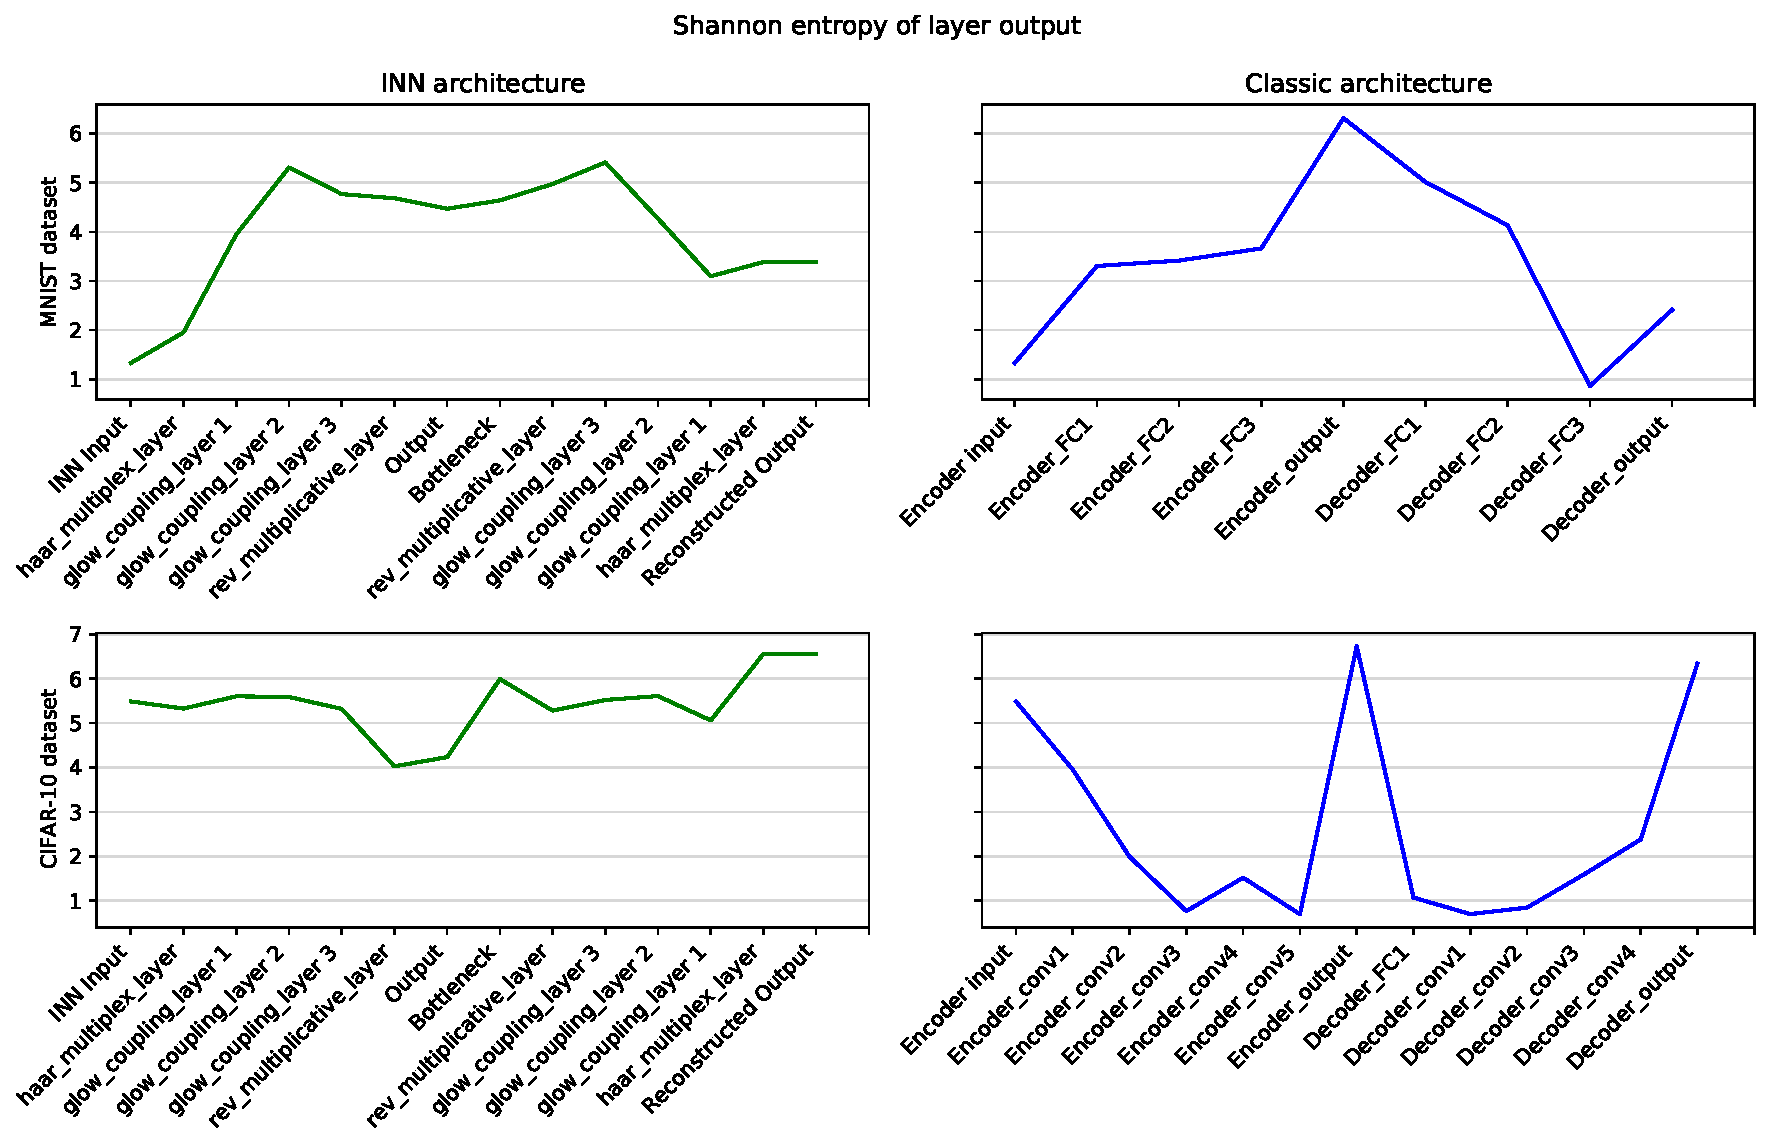
\includegraphics[height=10cm]{./pics/layer_entropies.pdf}
     \end{center}
     \end{figure}
     Figure 3 depicts the Shannon entropy of the output of each individual layer of the models.
     First, we examine the INN architectures.
     On MNIST, the entropy increases after the first two invertible coupling layers, then stays nearly constant, even after the bottleneck.
     Upon going through the model in reverse, the final two invertible coupling layers see the most decrease in entropy, and we find that our reconstructed output distribution has a slightly higher entropy than the original input distribution.
     On CIFAR-10, the entropy stays nearly constant, with the most noticeable spikes upon applying the bottleneck.
     This seems to indicate that on MNIST, the INN is more completely putting all useful information in the latent variable, whereas on CIFAR-10, there appears to be more information loss.

     The classic architecture shows very noticeable spikes at the \textit{Encoder\_output} layer, which indicates that we expect a high amount of information from the values at these layers.
     This is exactly what we expect, since the encoded output is intended to store all of the important information while discarding random noise.

     \subsubsection{Layer-wise Relative Entropy}
     \begin{figure}[!htb]
     \begin{center}
        \caption{}
        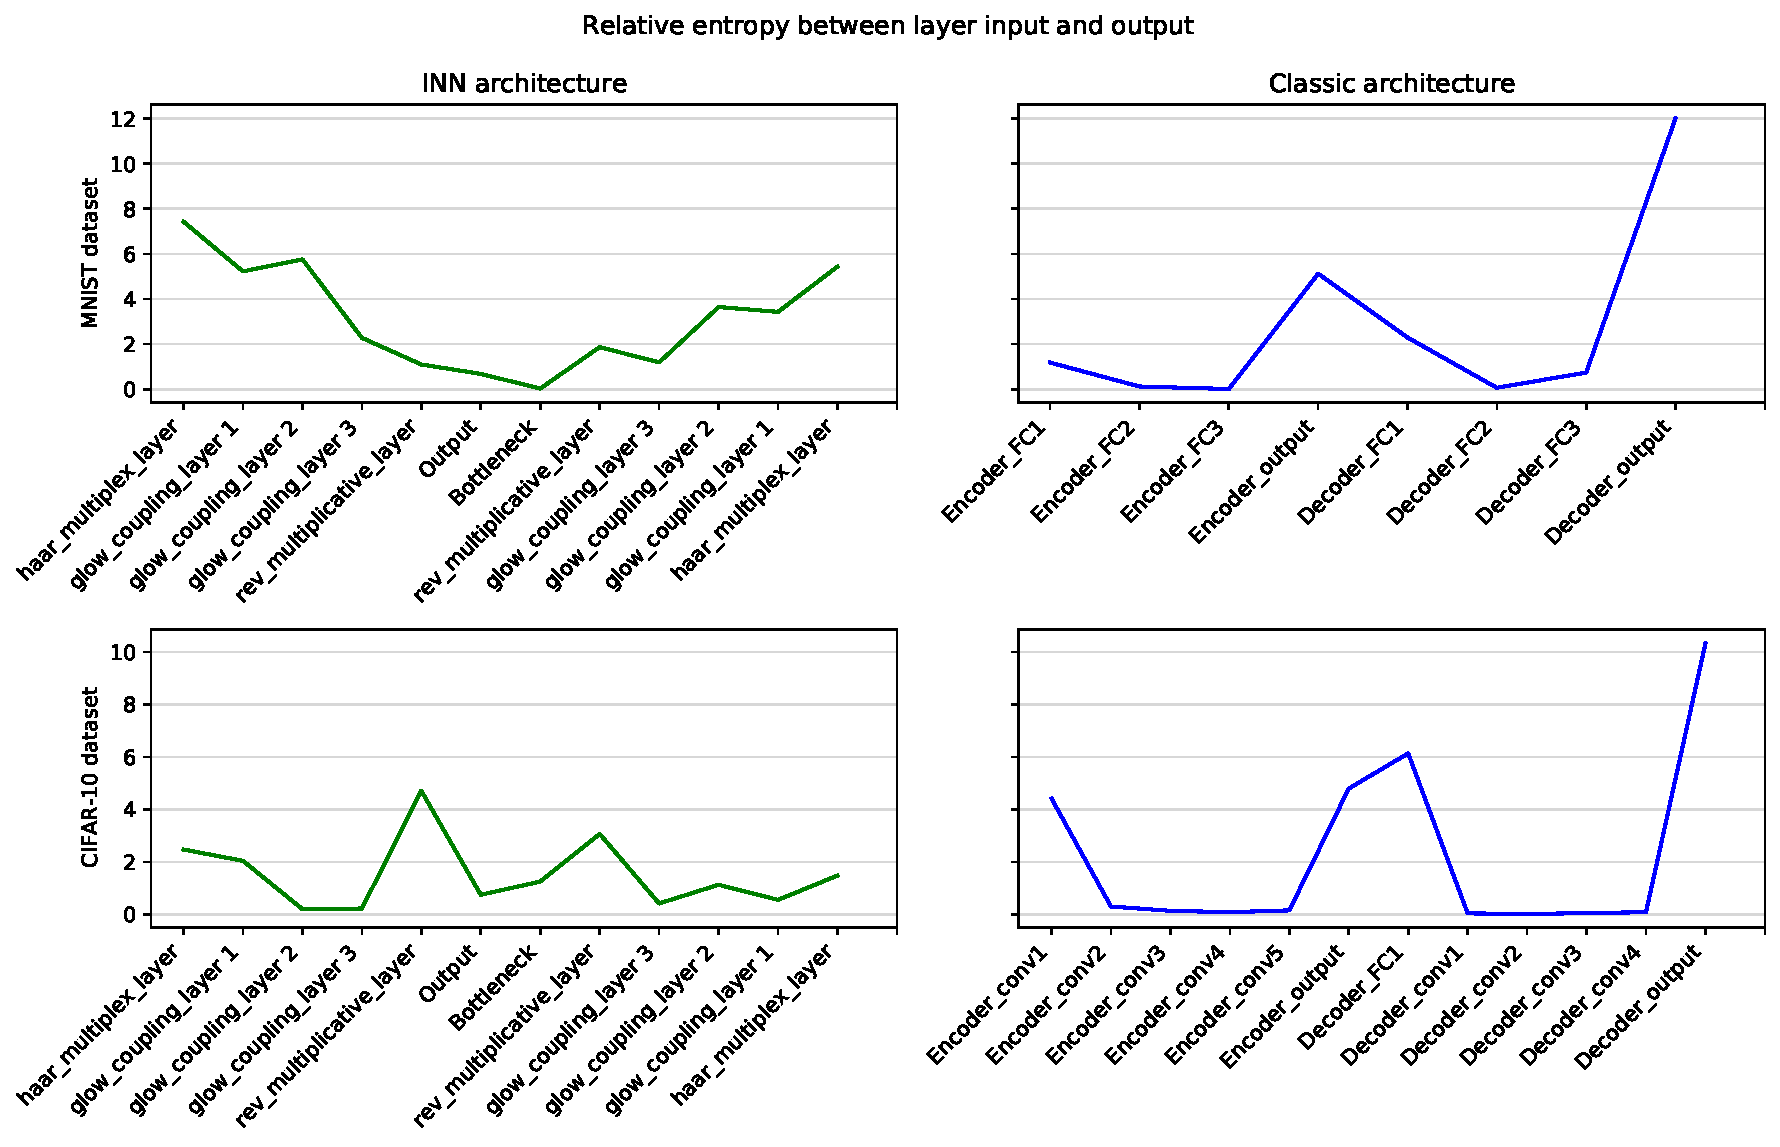
\includegraphics[height=10cm]{./pics/relative_entropies.pdf}
     \end{center}
     \end{figure}
      The results of this metric are more striking. We can see from Figure 4 that the relative entropies at each layer are much more constant in the INN autoencoders than they are in the classical autoencoders. Further, the classical autoencoders only see significant relative entropy values at the bottleneck layers and the output layers. This suggests that while both styles of autoencoder do a good job of preserving information from layer to layer, the classical autoencoder does it in an uneven way, providing almost no distributional change at non-bottleneck layers, and packing most of the distributional change into the bottleneck and outputs. In contrast, the INN autoencoder loses information at a more constant rate.

     \subsubsection{Relative entropy between inputs and outputs}
      The relative entropies between the inputs and outputs of each model are:
      \begin{center}
          \begin{tabular}{||c c c||}
          \hline
          Dataset & INN & Classical \\ [0.5ex]
          \hline\hline
          MNIST & 10.46 & 10.25 \\
          \hline
          CIFAR-10 & 0.76 & 0.28\\
          \hline
      \end{tabular}
      \end{center}
      It is clear to see that the relative information loss between input and output is very similar for each model. Surprisingly, the INN performs worse across both datasets. It is also interesting to note how drastically different the information loss is between the datasets. However, given that both the classical and INN architectures performed similarly on each dataset, it is probable that this discrepancy is due to properties of the datasets themselves and not the model architectures.

\section{Conclusion}
There are several interesting conclusions to draw from these results. First, it is clear that INN autoencoders do not preserve information as perfectly as hypothesized. In fact, they reconstruct images with information preservation similar to or worse than classical autoencoders. Interestingly, Nguyen et al. show that the reconstruction loss for INN autencoders is better than that of classical autoencoders. This suggests that the INNs could be overfitting more to the data while still losing a comparable amount of information.

 However, INN autoencoders seem to lose information at a more constant rate than do their classical counterparts, whose layer-wise entropy changes drastically depending on the layer. This means that on average the INN autoencoder loses less information across the intermediate layers. Given that the idea of an INN is to learn bijections, this behavior should be expected.

 In conclusion, it is clear that INN autoencoders handle information in a markedly different way than classical autoencoders, but it is not clear that they preserve any more information than their counterparts.

\bibliography{references.bib}{}
\bibliographystyle{plainnat}

\end{document}
